\documentclass[a4paper, 12pt]{report}
\usepackage[margin=1in]{geometry}
\usepackage{listings}
\usepackage[strings]{underscore}
\usepackage{dirtytalk}
\usepackage{xcolor}
\usepackage{multicol}
\usepackage{graphicx}
\usepackage{pdfpages}
\usepackage{appendix}
\usepackage{float}
\usepackage{hyperref}
\usepackage[acronym,toc]{glossaries}

\definecolor{comment}{RGB}{0,128,0} % dark green
\definecolor{string}{RGB}{255,0,0}  % red
\definecolor{keyword}{RGB}{0,0,255} % blue
\graphicspath{ {./images/} }

\loadglsentries{glossary}
\makeglossaries

\lstdefinestyle{c}{
	commentstyle=\color{comment},
	stringstyle=\color{string},
	keywordstyle=\color{keyword},
	basicstyle=\footnotesize\ttfamily,
	numbers=left,
	numberstyle=\tiny,
	numbersep=5pt,
	frame=lines,
	breaklines=true,
	prebreak=\raisebox{0ex}[0ex][0ex]{\ensuremath{\hookleftarrow}},
	showstringspaces=false,
	upquote=true,
	tabsize=2,
}

\lstdefinestyle{make}{
	commentstyle=\color{comment},
	stringstyle=\color{string},
	keywordstyle=\color{keyword},
	basicstyle=\footnotesize\ttfamily,
	numbers=left,
	numberstyle=\tiny,
	numbersep=5pt,
	frame=lines,
	breaklines=true,
	prebreak=\raisebox{0ex}[0ex][0ex]{\ensuremath{\hookleftarrow}},
	showstringspaces=false,
	upquote=true,
	tabsize=2,
}


%%%%%%%%%%%%%%%%%%
% TITLE
%%%%%%%%%%%%%%%%%%
\title{\Huge{\textbf{Using Blockchain to Create a Decentralised Security Model for Distributed Systems}}}
\date{April 2021}
\author{\Large{Adam David Bruce} \\ \texttt{\href{mailto:a.bruce3@newcastle.ac.uk}{a.bruce3@newcastle.ac.uk}}}
\begin{document}
\maketitle

%%%%%%%%%%%%%%%%%%
% ABSTRACT
%%%%%%%%%%%%%%%%%%
\begin{abstract}
//TODO
\end{abstract}

%%%%%%%%%%%%%%%%%%
% TABLE OF CONTENTS, FIGURES and TABLES
%%%%%%%%%%%%%%%%%%
\tableofcontents
\listoffigures
\listoftables

\newpage

%%%%%%%%%%%%%%%%%%
% INTRODUCTION
%%%%%%%%%%%%%%%%%%
\chapter{Introduction}
\section{COVID-19 and Cyberattacks}
In the summer of 2020 during the midst of the COVID-19 pandemic, universities and research institutions worldwide were working hard to understand the structure of the virus and develop a vaccine in an attempt to return to normality. However, whereas some countries were making fast progress in understanding the virus, others were falling behind, and the virus began to put a strain on healthcare, and increasing critique on governments. In order to keep up with the nations at the forefront of vaccine development, nations turned to state-sponsored cyberattacks in order to both hinder nations, and also obtain research and information about other countries' vaccine efforts. One such example was the threat group 'Cozy Bear', formally known as \acrfull{APT} 29. \acrshort{APT}29 used a number of tools to target various organisations involved in COVID-19 vaccine development in Canada, the United States and the United Kingdom. The \acrfull{NCSC} believe that the intention was highly likely stealing information and intellectual property relating to the vaccine \cite{APT29}.

In addition to the mortality of COVID-19, the virus also caused a number of economic issues across a number of nations. Global stock markets lost \$6 trillion in value over size days from 23 to 28 February \cite{covspill}. This gave private companies no other choice than to make large volumes of staff redundant, which increased job insecurity causing many people to become redundant, and in nations without suitable support or benefits, attackers turned to cybercrime for financial gain. These attacks represented the majority of cyberattacks aimed at both universities and the general public. A study of cyber-crime throughout the COVID-19 pandemic determined that 34\% of attacks directly involved financial fraud with a number of attack surfaces used, the majority being \gls{phishing}, \gls{smishing} and \gls{malware}~\cite{diffattack}.

University attacks became a frequent headline in the UK as universities suffered attacks from different threat actors. A number of threat actors launched attacks against multiple universities in the hope to find a vulnerability in at least one. One such attack was aimed at both Newcastle University and Northumbria University, two universities in extremely close proximity \cite{newhack,norhack}. The attack crippled both Newcastle and Northumbria Universities, however the attackers only managed to exfiltrate data from Newcastle University. Why was the attack successful on both occasions? Why wasn't knowledge of the attack shared? 

One reason is that currently, there is no reliable or automated system in place to share this information. Such a system is what this paper will aim to create. 

\section{Distributed Systems} \label{distributed}
A distributed system is defined by Tanenbaum and van Steen as a \say{collection of independent computers that appears to its users as a single coherent system} \cite{tanenbaumdist}. Such systems are commonplace in peer-to-peer computing and sensor networks where each systems contributes some data via transactions to the system. A distributed system therefore should be autonomous and to the user, should appear as though they are interacting with a single system. Furthermore users and applications should be able to interact with the distributed system in a consistent and uniform way, regardless of where and when system interaction takes place. This requires a common interface provided by a \gls{stub} which is used to bridge the gap between a programming language or protocol and the distributed system. This \gls{stub} hides the differences in machine architecture and communication between the computer and the distributed system. The use of \gls{stub}s creates a new software layer, known as \gls{middleware} which runs on an \acrfull{OS} and exposes distributed functions to higher-level applications and users.

\section{Decentralised Systems}
Reed defines a decentralised computer system as a computer system that \say{involves separation of the computers in the system by physical distance, by boundaries of administrative responsibility for individual computers and their applications, and by firewalls} \cite{namingSyncDec}. Reed suggests that for a computer system to be decentralised, it must be separated by both physical distance and administrative responsibility, such that no single body administrates the system. One of the most well-known examples of decentralisation is \gls{cryptocurrency}, a currency which takes no physical form, but instead exists entirely digitally. If cryptocurrency were to be governed by a central body, nefarious transactions could be used to launder money. Using a decentralised system ensures the transaction can only take place if all nodes within the system are in consensus that the transaction is genuine.

\begin{center}
	\begin{figure}[!htb]
		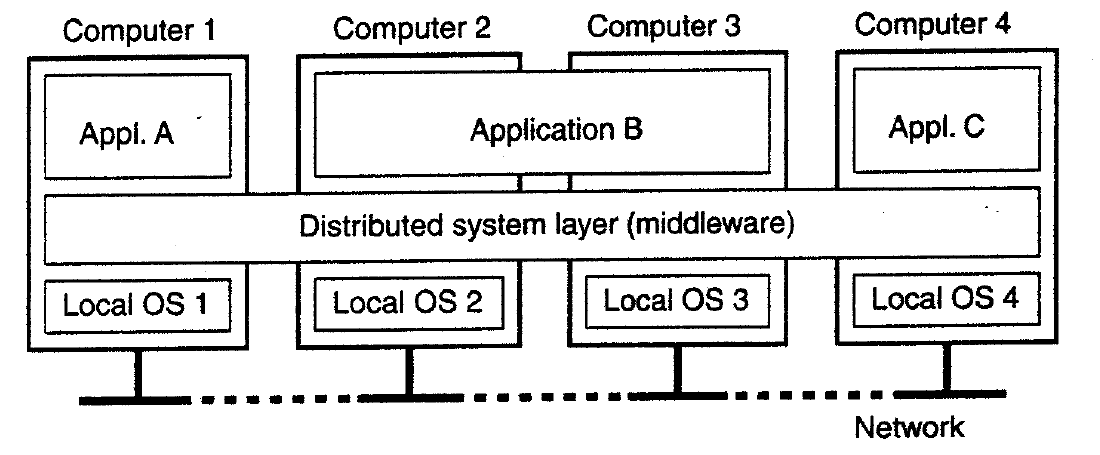
\includegraphics[width=\textwidth,keepaspectratio]{TanenbaumDistributed}
		\caption{A Distributed System visualised as \gls{middleware} \cite{tanenbaumdist}} 
		\label{fig:middleware}
	\end{figure}
\end{center}

\section{Blockchain}
Nofer et al. define \gls{blockchain}s as \say{data sets which are composed of a chain of data packages (blocks) where a block comprises multiple transactions. The \gls{blockchain} is extended by each additional block and hence represents a complete \gls{ledger} of the transaction history.} \cite{blockchain}. Nofer et al. describe the basic fundamentals of a \gls{blockchain}, which is that numerous blocks of transactions contribute to a larger chain. This chain is never controlled by a single body, instead a copy of the chain is stored at each node within a system, making \gls{blockchain} a popular candidate for controlling transactions over a decentralised computer system. Hence, \gls{blockchain} is the foundation for the vast majority of cryptocurrencies including Bitcoin\cite{bitcoin} and Ethereum\cite{ethereum}. One of the key aspects of \gls{blockchain} is the use of cryptographic \gls{hashing} algorithms, these algorithms represent a block as a fixed-length string. For a block to be added to the chain, it must contain the hash of the previous block.

\begin{center}
	\begin{figure}[H]
		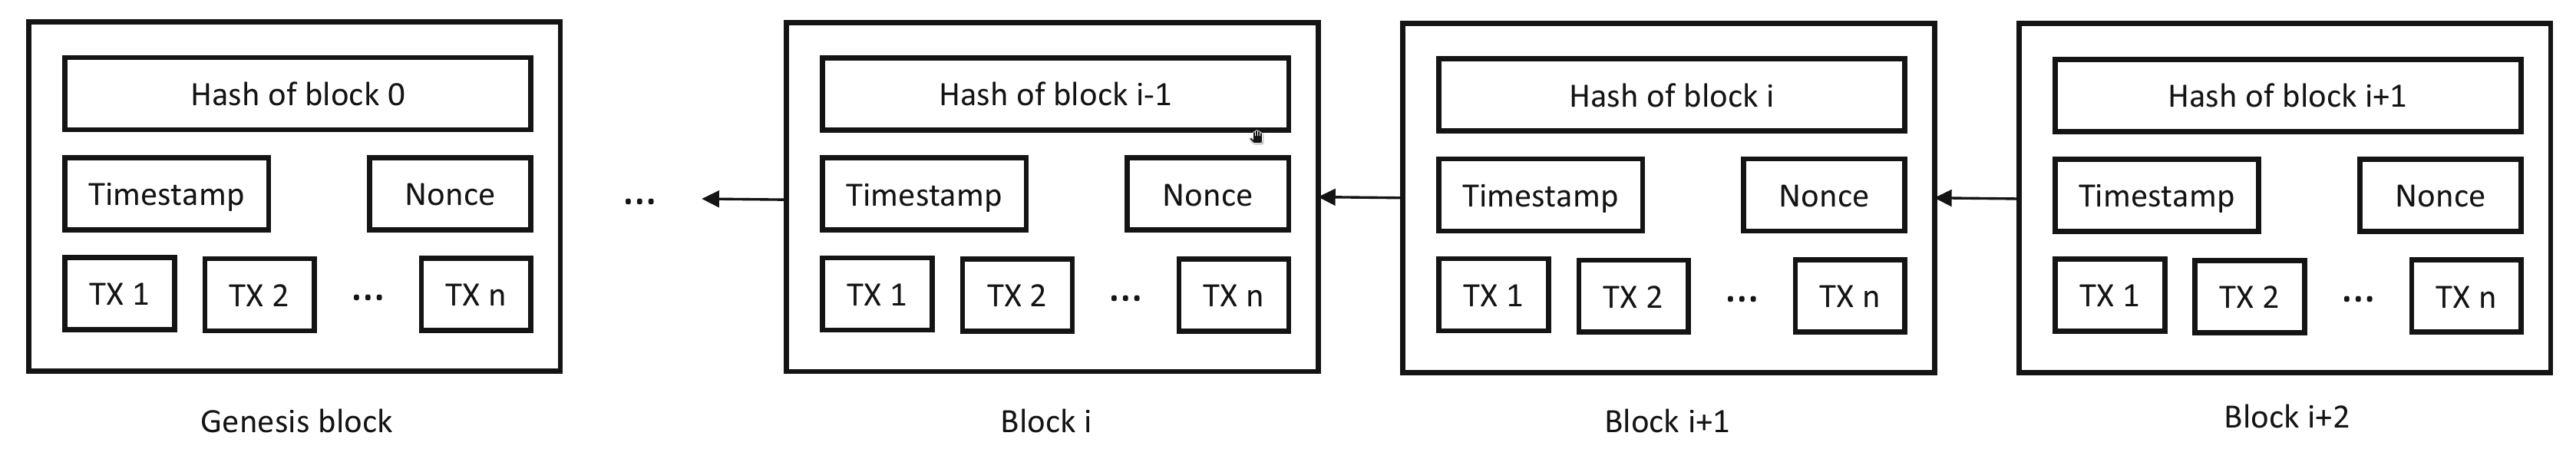
\includegraphics[width=\textwidth,keepaspectratio]{NoferBlock}
		\caption{An example of a \gls{blockchain} \cite{blockchain}} 
		\label{fig:middleware}
	\end{figure}
\end{center}

%%%%%%%%%%%%%%%%%%
% AIMS AND OBJECTIVES
%%%%%%%%%%%%%%%%%%
\chapter{Project Aims and Objectives}

\section{Aim}
The original aim for this project was to design and create a decentralised firewall that could communicate knowledge of cyberattacks aimed at universities in real-time, allowing other universities to protect themselves from the same attacks. This system would be distributed, and hence must conform to the previous description of a distributed system in section \ref{distributed}. Following an extensive amount of background reading, there appeared to be no existing implementation or design of such a system which inspired me to alter my aim and instead focus entirely on designing a protocol and implementing a \gls{stub} to demonstrate the protocol's effectiveness. This project will therefore not be implementing a firewall, but instead a system to coordinate firewalls. Further research determined that \gls{blockchain} was the best choice for the underlying structure for such a protocol, and so this final change shaped the current aim for this project: \textbf{Using Blockchain to Create a Decentralised Security Model for Distributed Systems}.

\section{Objectives}
The following objectives provide an outline for what this project hopes to achieve:

\begin{enumerate}
    \item Evaluate the effectiveness of existing distributed security mechanisms.
    \item Investigate methods of establishing connections and synchronising computers within distributed systems.
    \item Understand the structure of \gls{blockchain}s and adapt them for firewall transactions.
    \item Implement and rest relevant resilience, fault tolerance and security mechanisms.
    \item Compare the use of decentralised security mechanisms.
\end{enumerate}

%%%%%%%%%%%%%%%%%%
% BACKGROUND
%%%%%%%%%%%%%%%%%%
\chapter{Background}

\section{Distributed Systems}
The primary reference used for distributed systems was Tanenbaum and van Steen's \say{Distributed Systems: Principles and Paradigms}\cite{tanenbaumdist}, who's literature provides an in-depth explanation from the fundamental theory of distributed systems to the design and implementation of such systems. Key details that were taken from this publication are detailed below. In general, this book covered the essential components of creating a distributed system, however much of the detail with regards to client-server interactions was not applicable to this project due to it's decentralised nature. Furthermore, a large portion of the book was not of interest to this project as it focuses on distributed processing, which only comprises a small element of this project, hence a large volume of information regarding implementation of processing was not useful.

\subsection{Architecture}
Tanenbaum and van Steen cover many aspects of a distributed system's architecture spanning network, software and physical architecture. This project will implement a decentralised, peer-to-peer network architecture, which will be discussed in detail in section \ref{decentrailsed}. The software used will consist primary of \gls{stub}s, which are used to hide the differences in machine architecture and communication between the computer and the distributed system. The combined use of \gls{stub}s creates a new software layer, known as \gls{middleware} which provides a common interface between a client application, and the distributed system. Creating this layer enables applications to communicate via an application-level protocol, which is independent from the protocol spoken by the \gls{middleware}.

\begin{figure}[H]
\centering
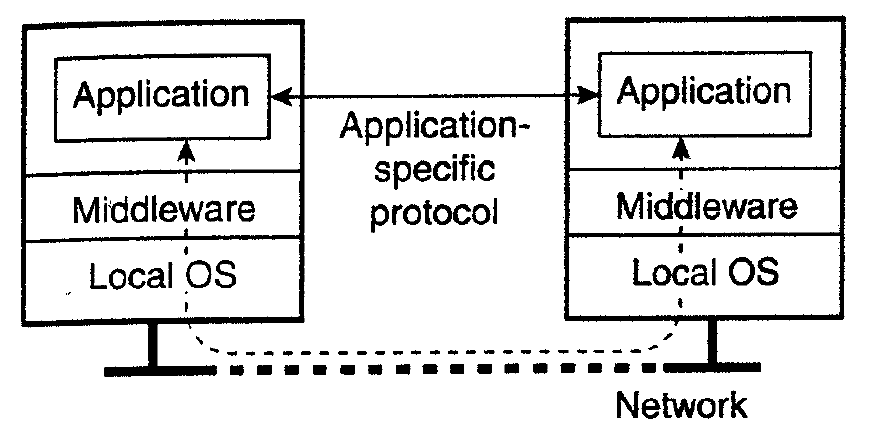
\includegraphics[height=5cm,keepaspectratio]{appl_layer_proto}
\caption{Application layer protocol running over \gls{middleware} \cite{tanenbaumdist}} 
\label{fig:middleware}
\end{figure}

With regards to physical architecture, Tanenbaum and van Steen discuss a number of approaches to client-server architectures, however due to the decentralised nature of this project, non of Tanenbaum and van Steen's classifications apply. 

\subsection{Remote Procedure Calls (RPC)}
Tanenbaum and van Steen introduce the concept of a \acrfull{RPC}. \acrshort{RPC}s are used to execute some action on a remote node within a distributed system.  Tanenbaum and van Steen provide a concise breakdown of the steps required to execute an \acrshort{RPC}:

\begin{enumerate}
    \item The client procedure calls the client \gls{stub} in the normal way.
    \item The client \gls{stub} builds a message and calls the local \acrfull{OS}.
    \item The client \acrshort{OS} sends the message to the remote \acrshort{OS}.
    \item The remote \acrshort{OS} gives the message to the server \gls{stub}.
    \item The server \gls{stub} unpacks the parameters and calls the server.
    \item The server does the work and returns the result to the \gls{stub}.
    \item The server \gls{stub} packs it in a message and calls it's local \acrshort{OS}.
    \item The server's \acrshort{OS} send the message to the client's acrshort{OS}.
    \item The client's \acrshort{OS} sends the message to the client \gls{stub}.
    \item The \gls{stub} unpacks the result and returns to the client.
\end{enumerate}

\begin{figure}[H]
\centering
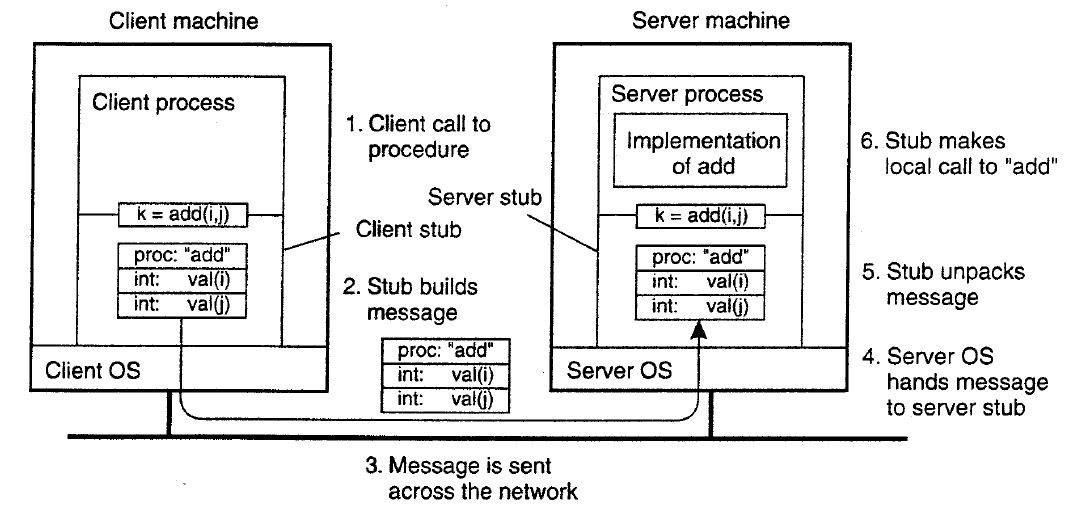
\includegraphics[width=\textwidth,keepaspectratio]{rpc}
\caption{A breakdown of an \acrshort{RPC} \cite{tanenbaumdist}} 
\label{fig:rpc}
\end{figure}

\section{Decentralised Systems} \label{decentrailsed}


\section{Blockchain}
The primary reference used for blockchain was Nofer et al.'s \say{Blockchain}\cite{blockchain}. 

\section{Distributed Security}

\section{Firewall Rules}

\section{Fault Tolerance}

\section{Inter-Process Communication (IPC)}

\printglossaries

\bibliography{bib} 
\bibliographystyle{ieeetr}

\appendix

%\iffalse
\chapter{Framework Source Code}
\lstinputlisting[language=c,style=c,caption=main.c,basicstyle=\ttfamily\scriptsize]{../src/main.c}
\lstinputlisting[language=c,style=c,caption=blockchain.h,basicstyle=\ttfamily\scriptsize]{../src/blockchain.h}
\lstinputlisting[language=c,style=c,caption=blockchain.c,basicstyle=\ttfamily\scriptsize]{../src/blockchain.c}
\lstinputlisting[language=c,style=c,caption=firewall.h,basicstyle=\ttfamily\scriptsize]{../src/firewall.h}
\lstinputlisting[language=c,style=c,caption=firewall.c,basicstyle=\ttfamily\scriptsize]{../src/firewall.c}
\lstinputlisting[language=c,style=c,caption=ipc.h,basicstyle=\ttfamily\scriptsize]{../src/ipc.h}
\lstinputlisting[language=c,style=c,caption=ipc.c,basicstyle=\ttfamily\scriptsize]{../src/ipc.c}
\lstinputlisting[language=c,style=c,caption=net.h,basicstyle=\ttfamily\scriptsize]{../src/net.h}
\lstinputlisting[language=c,style=c,caption=net.c,basicstyle=\ttfamily\scriptsize]{../src/net.c}
\lstinputlisting[language=c,style=c,caption=socket.h,basicstyle=\ttfamily\scriptsize]{../src/socket.h}
\lstinputlisting[language=c,style=c,caption=socket.c,basicstyle=\ttfamily\scriptsize]{../src/socket.c}

\chapter{Client Program Source Code}
\lstinputlisting[language=c,style=c,caption=client.c,basicstyle=\ttfamily\scriptsize]{"../src/example\string_client/client.c"}

\chapter{Code and Framework Documentation}
\includepdf[pages=-]{../docs/latex/refman.pdf}
%\fi

\end{document}